% REMEMBER: You must not plagiarise anything in your report. Be extremely careful.

\documentclass{l4proj}


%
% put any additional packages here
%
\usepackage{bm}
\usepackage{booktabs}

\begin{document}

%==============================================================================
%% METADATA
\title{Deep neural networks for classification of hyperspectral images}
\author{Niklas Lindorfer}
\date{September 26, 2019}

\maketitle

%==============================================================================
%% ABSTRACT
\begin{abstract}
    Every abstract follows a similar pattern. Motivate; set aims; describe work; explain results.
    \vskip 0.5em
    ``XYZ is bad. This project investigated ABC to determine if it was better. 
    ABC used XXX and YYY to implement ZZZ. This is particularly interesting as XXX and YYY have
    never been used together. It was found that  
    ABC was 20\% better than XYZ, though it caused rabies in half of subjects.''
\end{abstract}

%==============================================================================

% EDUCATION REUSE CONSENT FORM
% If you consent to your project being shown to future students for educational purposes
% then insert your name and the date below to  sign the education use form that appears in the front of the document. 
% You must explicitly give consent if you wish to do so.
% If you sign, your project may be included in the Hall of Fame if it scores particularly highly.
%
% Please note that you are under no obligation to sign 
% this declaration, but doing so would help future students.
%
\def\consentname {Niklas Lindorfer} % your full name
\def\consentdate {26 September 2019} % the date you agree
%
\educationalconsent


%==============================================================================
\tableofcontents

%==============================================================================
%% Notes on formatting
%==============================================================================
% The first page, abstract and table of contents are numbered using Roman numerals and are not
% included in the page count. 
%
% From now on pages are numbered
% using Arabic numerals. Therefore, immediately after the first call to \chapter we need the call
% \pagenumbering{arabic} and this should be called once only in the document. 
%
% The first Chapter should then be on page 1. You are allowed 40 pages for a 40 credit project and 20 pages for a 
% 20 credit report. This includes everything numbered in Arabic numerals (excluding front matter) up
% to but excluding the appendices and bibliography.
%
% You must not alter text size (it is currently 10pt) or alter margins or spacing.
%
%
%==================================================================================================================================
%
% IMPORTANT
% The chapter headings here are **suggestions**. You don't have to follow this model if
% it doesn't fit your project. Every project should have an introduction and conclusion,
% however. 
%
%==================================================================================================================================
\chapter{Introduction}

% reset page numbering. Don't remove this!
\pagenumbering{arabic} 


Why should the reader care about what are you doing and what are you actually doing?



%==================================================================================================================================
\chapter{Background}
What did other people do, and how is it relevant to what you want to do?


%==================================================================================================================================
\chapter{Analysis/Requirements}
What is the problem that you want to solve, and how did you arrive at it?



%==================================================================================================================================
\chapter{Design}
How is this problem to be approached, without reference to specific implementation details? 


%==================================================================================================================================
\chapter{Implementation}
What did you do to implement this idea, and what technical achievements did you make?

\section{Image registration: aligning the RGB and FIR images}

The images captured by the visible light camera and thermal sensor of the FLIR One Pro are not properly aligned by default. This can have adverse consequences to the classification performance of a machine learning model (XXX citation needed). Thus, an algorithm for properly aligning the images captured by the conventional camera and FIR camera had to be developed. The process of transforming data from different sensors into one coordinate system is commonly referred to as image registration.

On superficial inspection, it is apparent that the FIR sensor appears to have a larger focal length than the RGB camera, and therefore has a narrower field of view. Hence, an attempt was made to manually align the FIR and RGB images by cropping and rescaling the RGB image, effectively "zooming in". This approach yielded moderate results, as can be seen in (XXX).

To obtain a more flexible and generalisable representation, we made use of affine transformations. An affine transformation or affine map can accurately represent a composition of a translation and a linear map (e.g. scaling, rotation and shearing). A transformation $f(\vec{x})$ can be expressed as follows:

\begin{equation}
  f(\vec{x}) = A \vec{x} + \vec{b},
\end{equation}

where $\vec{x}$ represents the coordinates of a point to be translated, $A$ is a $2 \times 2$ linear map, and $\vec{b}$ is the translation vector.

Subsequently, the coordinates of about a dozen reference points were manually determined on the RGB and FIR versions of some test images. These coordinates were used as inputs and outputs to train a linear regression model representing the affine transformation required align the RGB image with the FIR image. 

The effect of applying the resulting transformation to a set of coordinates are shown in Figure \ref{fig:transformation_arrows}.

\begin{figure}[h]
  \centering
  \begin{subfigure}[h!]{0.45\textwidth}
    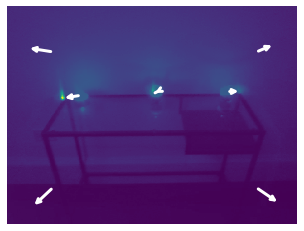
\includegraphics[width=\textwidth]{images/registration/transformation_arrows.png}
    \caption{Synthetic image, black on white.}
    \label{fig:transformation_arrows}
  \end{subfigure}
  
  \caption{}
\end{figure}

\begin{figure}[h]
  \centering
  \begin{subfigure}[h!]{0.9\textwidth}
    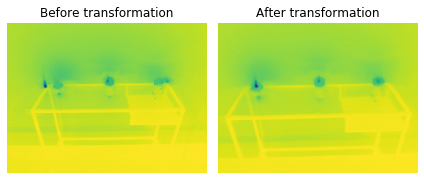
\includegraphics[width=\textwidth]{images/registration/linear_model_alignment.png}
    \caption{Synthetic image, black on white.}
    \label{fig:linear_trans_before_after}
  \end{subfigure}
\end{figure}

\subsection{Intensity-based registration metrics}

As can be seen in Figure \ref{fig:linear_trans_before_after}, the the candles on the images now line up. To quantify the accuracy of the alignment, attempts were made to use various metrics for image similarity. This task is difficult, as the properties of objects are vastly different under visible light and far infrared. Therefore, a simple intensity-based metric is unlikely to be robust in this scenario, as local intensities will vary across different channels even if the registration is perfect \citep{myronenko_intensity-based_2010}.

To mitigate this problem \citet{chen_normalized_2018} introduce the Normalized Total Gradient (NTG) metric for multispectral imaging systems, which is defined as follows:

\begin{equation}
  NTG(f, f_R) = \frac{\sum_l |\nabla_l \{f - f_R\}|}{\sum_l | \nabla_l f | + \sum_l | \nabla_l f_R|},
\end{equation}

where $f$ and $f_R$ are the channel images to be compared, $\nabla_l$ represents the gradient computation along the direction $l \in \{x, y\}$, and $| \cdot |$ denotes the L1-norm.

In other words, to obtain NTG one computes the sum of the $x$- and $y$-gradients of the difference of the two channels, and normalises the result by dividing over the sum of gradients of the individual channels.

The metric is based on the assumption that the gradient of the channel difference image becomes sparser as the alignment improves. Figure \ref{fig:gradient_distribution} shows that this is hardly the case for images captured by the FIR camera, as opposed to the baseline of comparing the red and green channels from the RGB camera.

This might be due to the fact that the resolution of output FIR files is $640 \times 420$ px, although the actual resolution of the sensor is only $160 \times 120$. Thus, when downsampling the RGB image to $640 \times 420$ px, edges are still much sharper than for the corresponding FIR image. Downsampling both images to the native resolution of the FIR camera did not yield better results.

Moreover, an attempt at smoothing both images before calculating the NTG was made by applying the Laplacian of Gaussian (LoG) with $\sigma=2$ to both images. As can be seen in Table \ref{table:registration_ntg}, this approach was not successful either. 

Considering these results, it can be concluded that NTG is not a suitable metric for this particular problem. As the baseline seems to work, it is possible that the properties of the FIR and RGB channels are too different for an intensity-based approach.

\begin{figure}[h]
  \centering
  \begin{subfigure}[h!]{0.45\textwidth}
    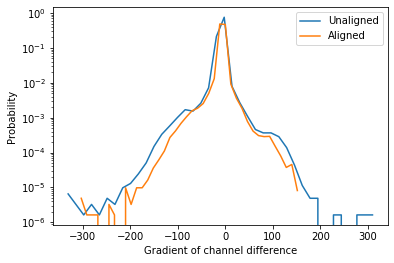
\includegraphics[width=\textwidth]{images/registration/gradient_distribution.png}
    \caption{LAB intensity of visible light image vs thermal intensity at $640 \times 420$ px}
    \label{fig:gradient_distribution}
  \end{subfigure}
  \begin{subfigure}[h!]{0.45\textwidth}
    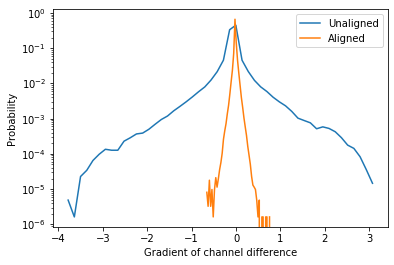
\includegraphics[width=\textwidth]{images/registration/gradient_distribution_red_green.png}
    \caption{Red channel intensity vs green channel intensity at $640 \times 420$ px}
    \label{fig:gradient_distribution_red_green}
  \end{subfigure}
  \caption{Distribution of gradients of the channel difference image before and after alignment using affine transformation.}
\end{figure}


\begin{table}[]
  \centering
  \begin{tabular}{@{}lll@{}}
  \toprule
  \textbf{Test configuration}                             & \textbf{Misaligned} & \textbf{Aligned} \\ \midrule
  LAB intensity of RGB vs FIR (640x480)     & 0.9984              & 0.9987           \\
  LAB intensity of RGB vs FIR (160x120)    & 0.9974              & 0.9986           \\
  LAB intensity of RGB vs FIR (after LoG with $\sigma=2$) & 0.9970              & 0.9973           \\
  (Baseline) Red vs green channels of RGB (160x120)                  & 0.6245              & 0.0303           \\ \bottomrule
  \end{tabular}
  \caption{Normalized Total Gradient before and after channel alignment}
  \label{table:registration_ntg}
\end{table}




%==================================================================================================================================
\chapter{Evaluation} 
How good is your solution? How well did you solve the general problem, and what evidence do you have to support that?



%==================================================================================================================================
\chapter{Conclusion}    
Summarise the whole project for a lazy reader who didn't read the rest (e.g. a prize-awarding committee).

%==================================================================================================================================
%
% 
%==================================================================================================================================
%  APPENDICES  

\begin{appendices}

\chapter{Appendices}

Typical inclusions in the appendices are:

\begin{itemize}
\item
  Copies of ethics approvals (required if obtained)
\item
  Copies of questionnaires etc. used to gather data from subjects.
\item
  Extensive tables or figures that are too bulky to fit in the main body of
  the report, particularly ones that are repetitive and summarised in the body.

\item Outline of the source code (e.g. directory structure), or other architecture documentation like class diagrams.

\item User manuals, and any guides to starting/running the software.

\end{itemize}

\textbf{Don't include your source code in the appendices}. It will be
submitted separately.

\end{appendices}

%==================================================================================================================================
%   BIBLIOGRAPHY   

% The bibliography style is abbrvnat
% The bibliography always appears last, after the appendices.

\bibliographystyle{abbrvnat}

\bibliography{l4proj}

\end{document}
